\documentclass{article}
\usepackage{pdfpages}
\usepackage{amsmath}
\usepackage[margin=.8in]{geometry}


\begin{document}
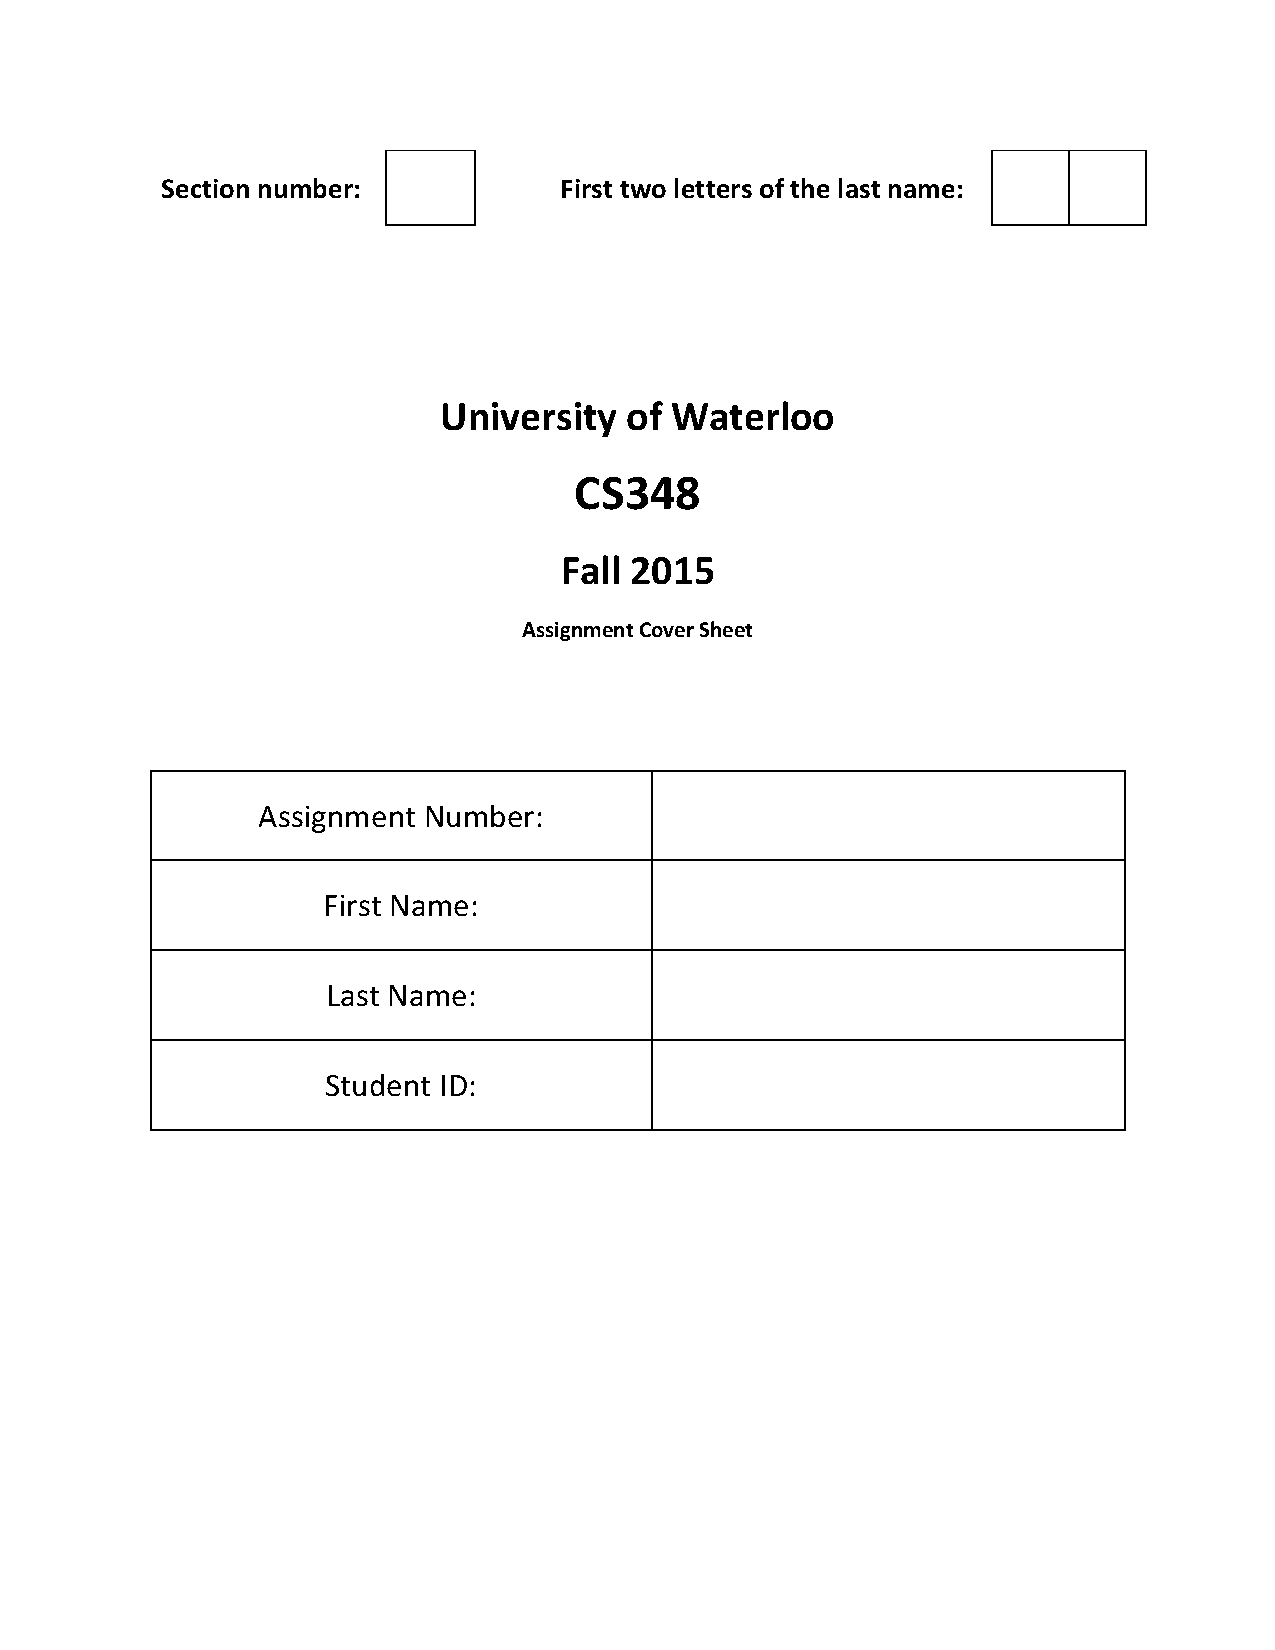
\includepdf[pages={1}]{../assignment_cover_sheet.pdf}


% 1. Find the names of employees who borrow a book that is published by McGraw-Hill or is published by Wesley.
% 2. Find all tuples <e1, e2, isbn> such that e1 and e2 are distinct empno and both employees borrow the same book isbn in Loan relation at some point of time.
% 3. Find the empno and the age of the oldest employees in the Employee relation.
% 4. Find the names of employees who borrow all books authored by Agatha Christie. You may assume Agatha Christie authored at least one book in the Book relation, and there is exactly one name in the author of the Book relatio



\section*{Question 1}
\begin{align*}
    \text{PUBLISHED} &= \sigma_{\text{PUBLISHER='McGrawHill' AND PUBLISHER='Wesley'}}(\text{BOOKS})\\
    \text{PUB\_LOANS} &= \text{PUBLISHED} * \text{LOAN}\\
    \text{PUB\_EMP} &= \text{PUB\_LOANS} * \text{EMPLOYEE}\\
    \text{ANSWER} &= \pi_{name}(\text{PUB\_EMP})
\end{align*}
The PUBLISHED table is a table of all books that have been published by the given publishers found through the select function. The PUB\_LOANS table joins the LOAN table with the PUBLISHED table to get the empno of the employees that borrowed the books by the given publishers. The PUB\_EMP table joins the EMPLOYEE table with the PUB\_LOANS table to get the employee information relating to the empno correspoding with books by the given publishers. Finally we get the answer by using the projection function to grab only the name column of the PUB\_EMP table. This should be the names of employees who have a empno corresponding with a loan whose isb corresponds to a book by one of the given publishers.

\section{Question 2} % (fold)
\label{sec:question_2}
\begin{align*}
    \text{EMPISBN} &= \pi_{empno,isbn}(\text{LOANS})\\
    \text{DUPLICATE} &= \rho_{empno2,isbn}(\text{EMPISBN})\\
    \text{SAMEBOOK} &= \text{EMPISBN} * \text{DUPLICATE}\\
    \text{ANSWER} &= \sigma_{empno!=empno2}(SAMEBOOK)\\
\end{align*}
The table EMPISBN is just the LOANS table with the empno and isbn columns removed since they are the only ones of relevance. We use this new table to create a DUPLICATE table that contains all of the same information, but renames the emplno column to empno2. This is done so that the SAMEBOOK table can be formed by taking the natural join of EMPISN and DUPLICATE table. This will create a row for all rows in the EMPISBN table that have the same isbn value (since the DUPLICATE table has duplicate data but renamed the empno column to prevent the join from matching on it and removing duplicates). The SAMEBOOK table contains duplicates because each loan will match with itself, so we remove these duplicates using the sigma operator (remove all entries where both empnos are the same) to get the answer.
% section question_2 (end)



\section*{Question 3} % (fold)
\label{sec:question_3}
\begin{align*}
    \text{EMPAGE} &= \pi_{\text{empno,age}}(\text{EMPLOYEE})\\
    \text{AGES} &= \rho_{age2}(\pi_{age}(\text{EMPLOYEE}))\\
    \text{NOTMAX} &= \pi_{empno,age}(\sigma_{age<age2}(\text{EMPAGE} \times \text{AGES}))\\
    \text{ANSWER} &= \text{EMPAGE} - \text{NOTMAX}\\
\end{align*}
The EMPAGE table is just a table of empnos and their corresponding ages since these are the only values that matter. The AGES table is a secondary table of just the ages of all employees renamed to age2. We use these two tables to create a table comparing all employees ages against all other ages by taking their cartesian cross. When this table is filtered by having age less than age2 we get a list of all employees that are younger than someone. The NOTMAX table is this table of employees that are younger than someone, taking only the age and empno columns (since age2 is no longer relevent). By taking the set difference of EMPAGE (the table with all employees number and ages) and NOTMAX (the table of all employees younger than someone's numbers and ages) we should get the employee that is not younger than anyone and this the oldest.
% section question_3 (end)

\section*{Question 4} % (fold)
\label{sec:question_4}
\begin{align*}
    \text{ALLCHRISIE} &= \sigma_{\text{AUTHOR='Agatha Christie'}}(\text{BOOKS}\times \text{EMPLOYEE})\\
    \text{NOTALLCHRISTIE} &= \pi_{empno,isbn}(\text{ALLCHRISTIE}) - \pi_{empno,isbn}(\text{LOANS})\\
    \text{ANSWER} &= \pi_{name}(\text{EMPLOYEE}) - \pi_{name}(\text{NOTALLCHRISTIE})
\end{align*}

The ALLCHRISTIE table is a table representing what would happen if all employees had checkedout all Agatha Christie books. This is found by taking the cartesian product of the BOOKS table and EMPLOYEE table and filtering on books where the author was Agatha Christie. Then a table is made for all employee-book combinations that were not checked out by subtracting the LOANS table from the ALLCHRISTIE table to form the NOTALLCHRISTIE table (both tables are narrowed to empno and isbn to make the subtraction work). This NOTALLCHRISTIE table should now contain all employees and the Agatha Christie books that they did not checkout. By taking just the names column of this table we have a list of all employees that have not checkout out all Agatha Christie books, so the answer can be found by subtracting this list from a list of all employees.
% section question_4 (end)

\end{document}
